\chapter{Einlesen von Signalen}

\begin{lstlisting}
#include "codeclib.h"
#include "copydata.h"


/* 	@function 	copyData
* 	@brief 		Kopiert die Audiodaten des Kanals "Internal ADC R0" aus 
*              dem DMA-Lesepuffer in den Speicherbereich iInput schreibt. 
* 	@param 		input	Adresse der ersten Speicherstelle von input 
*	@param 		pWrite	Zeiger auf die Adresse von input
*	@param 		size 	Anzahl der übergebenen Werte
*	@return 	void
*/
void copyData(int *input, int **pWrite, int size) {    

	// Nimm den 5ten Wert aus iDMARxBuffer und schreibe diesen in den input.
	**pWrite = iDMARxBuffer[4];
	
	// Inkrementiere den Wert der zuletzt beschriebenen Adresse
	(*pWrite)++;
	
	// Wenn die obere Grenze size erreicht wurde müssen wir auf die 
	// Startadresse zurückspringen.
	if(*pWrite == input + size)
	{
		*pWrite = input;
	}

}
\end{lstlisting}

Hier zu sehen Bilder, wow!

\begin{center}
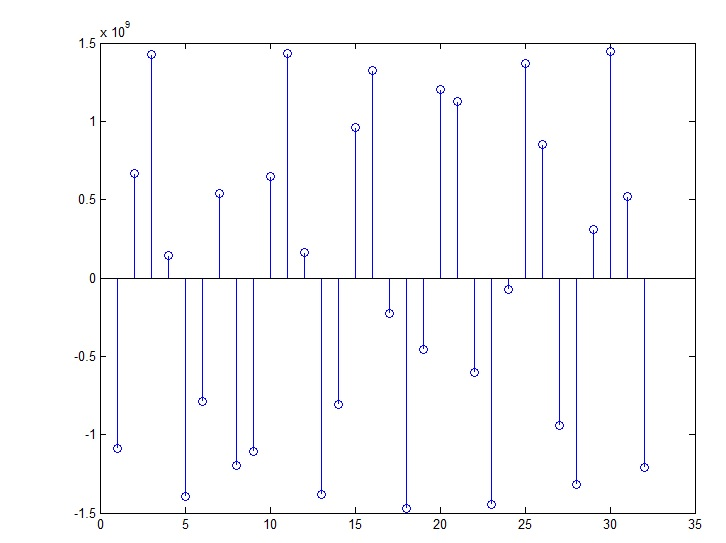
\includegraphics[scale=0.8]{Aufgabe1Matlab1.jpg}
\label{fig.Matlab}
\end{center}
